\documentclass[12pt]{article}
\usepackage[utf8]{inputenc}
\usepackage{amsmath, amssymb,multicol}
\usepackage{hyperref}
\usepackage{tikz}
\usepackage[left=2.5cm,right=2.5cm,bottom=2.5cm]{geometry}
\usetikzlibrary{arrows, arrows.meta, positioning, bending, quotes}
\hypersetup{
    colorlinks=true}

\title{MATH 5707 (Spring 2026): Homework 10}
\date{}

\begin{document}
\vspace{-0.7in}

\maketitle
\vspace{-0.6in}


\section*{Directions and Introduction}
Submit a pdf of your solutions to the HW 10 assignment on Gradescope by 11:59 pm on May 1.
\\[5pt]
\textbf{All of the problems in this assignment are optional. } They will only count towards the proficiency component of your final grade. Only submit the problems that use a skill  with which you still need to demonstrate proficiency.
\\[5pt]
Problem 3 is marked as a peer review problem. \href{https://docs.google.com/document/d/1jSw9pmMJJFUx_6dTkcUi4k4HJNIrrIIgs9zdWhAycx0/edit?usp=sharing}{This document gives directions and deadlines for the peer review process.}



\section*{Problems}

\begin{enumerate}
\item[0.] If you would like any of these problems to be graded for proficiency with the key skills, list the skill and the corresponding problem.  If you want to label the skill by number, use the numbering that is in the syllabus.

\item At least one of the following graphs is planar.   Pick one planar graph and prove that it is planar by drawing a plane embedding and proving that your plane embedding is, in fact, isomorphic to the graph you picked.  
\begin{center}
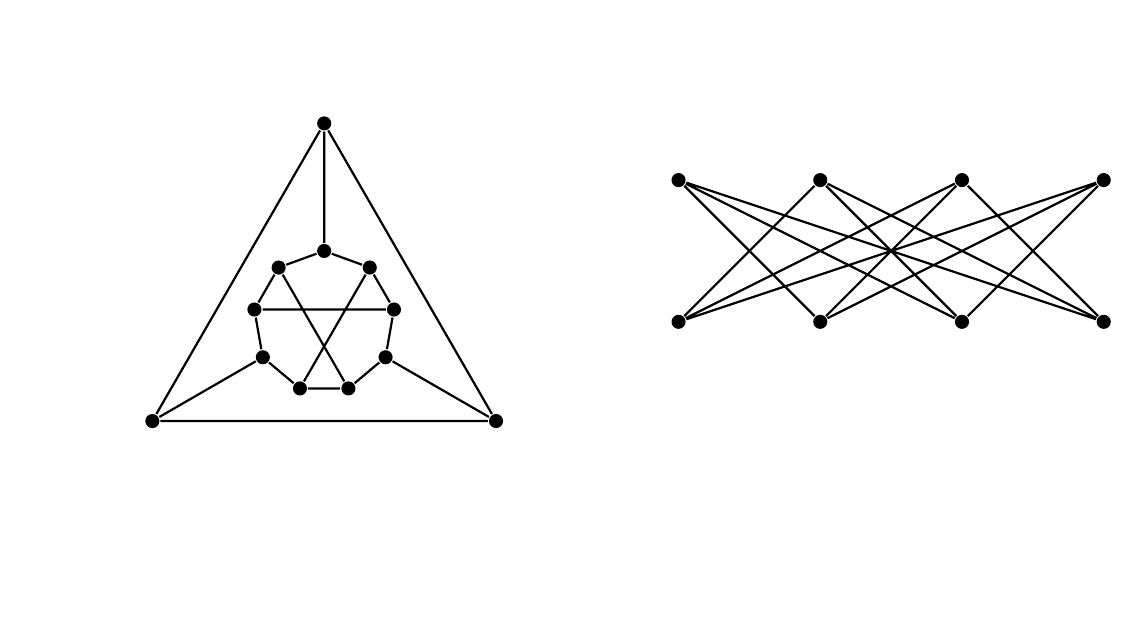
\begin{tikzpicture}[scale=1.8]
    \draw[thick,every node/.style={inner sep=1.8pt,fill,circle}]
    (-2.5,0) \foreach \x in {0,1,2,3,4,5,6,7,8}{+(90+40*\x:.5)node(x\x){}}
    (-2.5,0) \foreach \x in {0,1,2}
    {+(90+120*\x:1.4)node(y\x){}}
    (x0)--(x1)--(x2)--(x3)--(x4)--(x5)--(x6)--(x7)--(x8)--(x0)--(y0)--(y1)--(y2)--(y0) (y1)--(x3) (y2)--(x6) (x1)--(x5) (x2)--(x7) (x4)--(x8);
    \draw (-3.5,-2)node[white](){.} (-4.5,2)node[white](){.};

        \draw[thick,every node/.style={inner sep=1.8pt,fill,circle}] 
    \foreach \x in {0,1,2,3} {(\x,0) node(x\x){}}
    \foreach \y in {0,1,2,3} {(\y,1) node(y\y){}}
(x0)--(y1)--(x2)--(y3)--(x1)--(y0)--(x3)--(y2)--(x0)--(y2)--(x1)--(y3)--(x0)
(x2)--(y0)
(x3)--(y1)
;
    \end{tikzpicture}
\end{center}



\item Prove or disprove: If $G$ is planar and $G^*$ is the dual graph of $G$, then $(G^*)^*\cong G$. 
\item Draw a graph $G$ that satisfies the following properties, or explain why no such graph can exist.
\begin{enumerate}
\item A simple planar graph with degree sequence $\{4,4,4,5,5,5,6,6,6,7,7,7\}$.
\item A simple planar 4-regular graph.
\end{enumerate}

   
   \item (Peer review problem) Let $G$ be a plane embedding of a planar graph. Show that you can properly color the faces of $G$ in two colors if and only if $G$ is Eulerian.  (By properly color, we mean that, if two faces share an edge, they must be a different color.)
   
       \item You are the head of security at a major museum and you are trying to find the minimum number of guards needed to make sure that every hallway is under the direct line of sight of a guard.  
\begin{enumerate}
\item  To reframe this as a graph theory problem, we can let...
\begin{itemize}
\item Vertices represent \rule{1cm}{0.15mm}
\item Edges represent \rule{1cm}{0.15mm}
\item The chromatic number represents \rule{1cm}{0.15mm}
\end{itemize}
\item What statistic/property of the graph gives you the minimum number of guards necessary?
\end{enumerate}       
     \item (Bondy-Murty 2.1.8) For two vertices $u$ and $v$, define $d(u,v)$ to be the length of the shortest path between $u$ and $v$. A \emph{center} of $G$ is a vertex $u$ such that $\mathrm{max}_{v\in V} d(u,v)$ is as small as possible. Show that a tree has either exactly one center or two adjacent centers. 
 
\end{enumerate}

\end{document}